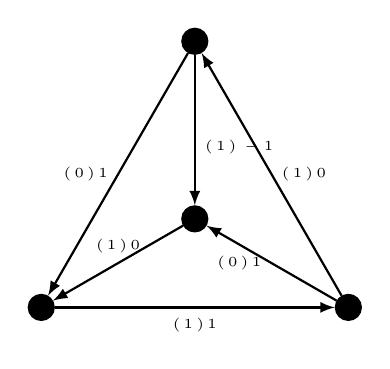
\begin{tikzpicture}[auto,scale=0.65]

	\node (c0) [circle, draw, fill=black] at (0, 0) {};
	\node (c1) [circle, draw, fill=black] at (6, 0) {};
	\node (c2) [circle, draw, fill=black] at (3, 5.2) {};
	\node (c3) [circle, draw, fill=black] at (3, 1.73) {};

	\path
	(c0) edge[-latex, thick] node[below] {\tiny $\begin{pmatrix}1 \\ 1\end{pmatrix}$} (c1)
	(c1) edge[-latex, thick] node[right] {\tiny $\begin{pmatrix}1 \\ 0\end{pmatrix}$} (c2)
	(c2) edge[-latex, thick] node[below right] {\tiny $\begin{pmatrix}1 \\ -1\end{pmatrix}$} (c3)
	(c2) edge[-latex, thick] node[left] {\tiny $\begin{pmatrix}0 \\ 1\end{pmatrix}$} (c0)
	(c3) edge[-latex, thick] node[above] {\tiny $\begin{pmatrix}1 \\ 0\end{pmatrix}$} (c0)
	(c1) edge[-latex, thick] node[left] {\tiny $\begin{pmatrix}0 \\ 1\end{pmatrix}$} (c3);
	
\end{tikzpicture}
